\chapter{Energía eléctrica y desarrollo sostenible.}

\section{Introducción al desarrollo sostenible.}
El desarrollo nació en los años 70 en los países nórdicos y se define como:
\begin{itemize}
	\item [-] El que satisface
	nuestras necesidades actuales sin poner en peligro la
	capacidad de las generaciones futuras para satisfacer sus
	propias necesidades abarcando:
	\begin{itemize}
		\item El capital social
		\item El capital ambiental
		\item El capital económico
	\end{itemize}
\end{itemize}
\subsection{Cumbres climáticas.}
\begin{itemize}
	\item [-] \textbf{Rio de Janeiro (1992):}
		Se crea la Comisión del Desarrollo Sostenible para impulsar la sostenibilidad de las políticas de desarrollo humano y gestionar sus riesgos.
	\item [-] \textbf{Cumbre del Protocolo de Kyoto (1997):}
		Se adquiere un compromiso entre los países industrializados con el \textbf{objetivo} de reducir las emisiones de gases de efecto invernadero un 5,9\% en el periodo 2008 - 2012 con respecto a 1990 (año base). En una fase inicial no incluía a países en desarrollo como China e India por su baja contaminación per capita.
	\item [-] \textbf{Cumbre de París (2015):}
		Se comprometen los países a que la temperatura mundial no aumente más de 2\textdegree C respecto a los niveles preindustriales y limitarlo a 1,5\textdegree C para el 2020.
	\item [-] \textbf{Cumbre de Marrakech (2016):}
		Se ratifican los acuerdos de la Cumbre de París y se compromete reducir el 80\% de las emisiones de CO$_2$ para 2050.
	\item [-] \textbf{Cumbre de Katowice (2018):}
		Limitar a un incremento a final de siglo de 1,5 a 2\textdegree C respecto a los niveles preindustriales.
	\item [-] \textbf{Cumbre de Chile celebrada en Madrid (2019):}
		Los grandes contaminadores se niegan a intensificar los esfuerzos para mantener la temperatura por debajo de 1,5\textdegree C.
	\item [-] \textbf{Cumbre de Glasgow (2021):}
		Se mantiene el objetivo de 1,5\textdegree C para 2030. Acuerdo China - USA para reducir las emisiones de metano. Compromiso de 130 países para poner fin a la deforestación.
	\item [-] \textbf{Cumbre de Sharm el-Sheij en Egipto (2022):}
		Se acuerdan:
		\begin{itemize}
			\item Una alianza global contra la sequía.
			\item Una coalición contra la deforestación.
			\item Impulsar el hidrógeno verde.
			\item Impulsar la energía eólica marina.
		\end{itemize}
	\item [-] \textbf{Cumbre de Dubai(2021):}
		Se acuerda reducir las emisiones mundiales de gases de efecto invernadero un 43\% hasta
		2030 y un 60\% hasta 2035 en relación con los niveles de 2019, y emisiones netas de dióxido de carbono cero
		para 2050.
\end{itemize}
\section{Gases de efecto invernadero.}
\subsection{CO$_2$ equivalente.}
Es una forma de poder reducir el impacto climático a una unidad común y así, poder compararlos. Para calcularlo se emplea el valor \textbf{GWP} (Global Warming Potencial) o \textbf{PCG} (Potencial de calentamiento global) que miden cuanto calor atrapan en comparación con el CO$_2$ para un periodo de tiempo. 


Este valor depende de:
\begin{itemize}
	\item [-] La absorción de radiación infrarroja.
	\item [-] La ubicación del espectro de absorción.
\end{itemize}
\subsection{Dióxido de carbono (CO$_2$).}
Es la sustancia que más contribuye al efecto invernadero. Absorbe gran parte de la radiación solar incidente.
\subsection{Óxido nitroso (N$_2$O) y óxidos de nitrógeno (NO$_x$ ).}
Son los gases de efecto invernadero más destructivos con la capa de ozono. Relacionados con el sector agrario y la quema de combustible.
\subsection{Metano (CH$_4$).}
Tiene un potencial de calentamiento muy elevado GWP = 25. Se emite por el sector ganadero, el de tratamiento de residuos y durante el transporte de hidrocarburos.
\subsection{Hidrofluorocarbonos (HFC).}
Son gases empleados como refrigerantes. No dañan al ozono pero tienen un GWP = 1000 y una larga permanencia en la atmósfera.
\subsection{Perfluororcarburos (PFC).}
Similares a los HFC.
\subsection{Hexafluoruro de azufre (SF$_6$).}
Se emplea para equipos de distribución de energía eléctrica. Tiene propiedades similares a los HFC y PFC.

\begin{table}[H]
	\centering
	\begin{tabular}{p{2cm}p{2cm}p{2cm}p{2cm}p{2cm}}
		\hline
		\textbf{ } & \textbf{CO$_2$} & \textbf{ClFCs} & \textbf{CH$_4$} & \textbf{N$_2$O} \\ \hline
		Importancia según contribución al efecto invernadero & Más del 50\% & 20 \% aprox. & 12 a 14 \% & 6 a 7 \% \\ \hline
		Tiempo de permanencia en la atmósfera & 50 - 200 años & 75 - 100 años & 7 a 10 años & 150 años aprox. \\ \hline
		Tasa de crecimiento anual (\%)&0,5&4-5&1&0,35\\ \hline 
		Principal origen de la contaminación&Combustión del petróleo, carbón y gas deforestación&Aerosoles y disolventes Espumas industriales Equipos de refrigeración&Pantanos Ganadería Minería&Fertilizantes Combustible fósiles\\ \hline 
	\end{tabular}
	\label{tab:my-table}
\end{table}

\section{Efecto invernadero.}
Como consecuencia de los gases de efecto invernadero se absorbe una mayor cantidad de radiación infrarroja que escaparía de la tierra y, por tanto, aumentando la temperatura atmosférica. 
\begin{figure}[H]
	\centering
	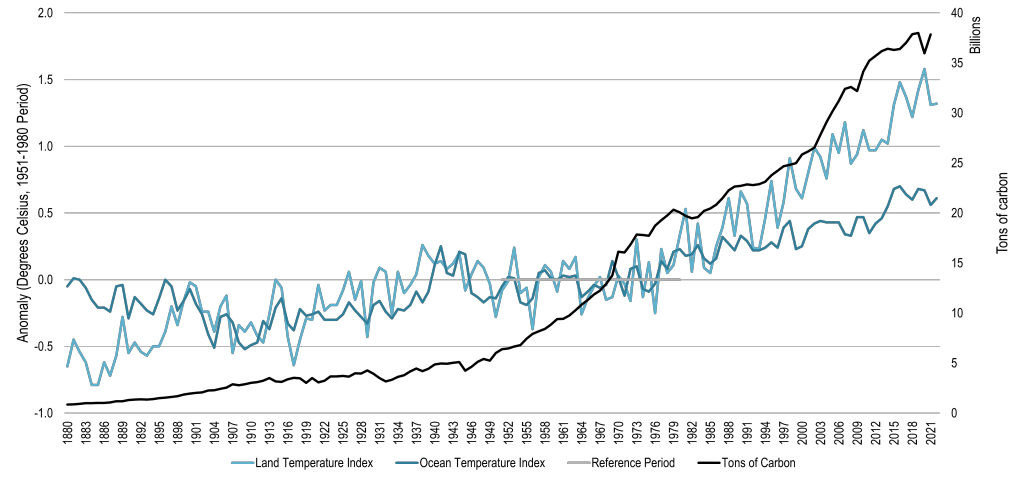
\includegraphics[width=0.7\linewidth]{res/tema2/T-Emisiones}
	\label{fig:t-emisiones}
\end{figure}
\subsection{Forzamiento radiactivo o climático.}
Es la diferencia entre la radiación solar absorbida por la Tierra y la energía irradiada de vuelta al espacio. Esta diferencia se contempla mediante el RCP donde:
\begin{itemize}
	\item [-] RCP = 2 es un escenario con el indicador muy bajo.
	\item [-] RCP = 8,5 es un escenario con el indicador muy alto.
\end{itemize}

\begin{table}[h]
	\centering
	\renewcommand{\arraystretch}{1.5}
	\begin{tabular}{cccccc}
		\hline
		Escenario & Forz. Radiat. (W/m\textsuperscript{2} en 2100) & \multicolumn{2}{c}{GC} & \multicolumn{2}{c}{GtCO$_2$} \\
		\cline{3-6}
		& &Media & Rango & Media & Rango \\
		\hline
		RCP2.6 & 2.8 & 270 & 140 a 410 & 990 & 510 a 1505 \\
		RCP4.5 & 4.5 & 780 & 595 a 1005 & 2880 & 2180 a 3690 \\
		RCP6.0 & 6 & 1060 & 840 a 1250 & 3885 & 3080 a 4585 \\
		RCP8.5 & 8.5 & 1685 & 1415 a 1910 & 6180 & 5163 a 7005 \\
		\hline 
	\end{tabular}
\end{table}

\begin{table}[H]
	\centering
	\renewcommand{\arraystretch}{1.5}
	\begin{tabular}{p{4cm}p{2cm}p{1cm}p{3cm}p{1cm}p{3cm}}
		\hline
		& \textbf{Escenario} &
		\multicolumn{2}{c}{\textbf{2046-2065}}  & \multicolumn{2}{c}{\textbf{2081-2100}} \\ 
	
		& &\textbf{Media} & \textbf{Rango probable} & \textbf{Media} &\textbf{Rango probable} \\ 
		\hline
		Cambio en la   & 
		RCP2,6 & 1 & 0,4 a 1,6 &1 &0,3 a 1,7\\
		temperatura media global&RCP4,5 & 1,4 & 0,9 a 2,0 &1,8 & 1,1 a 2,2 \\
		del aire en superficie & RCP6 & 1,3 & 0,8 a 1,8 & 2,2 & 1,4 a 3,1\\
		(en °C)& RCP8,5 & 2 & 1,4 a 2,6 & 3,7 & 2,6 a 4,8 \\
		\hline
		Elevación media mundial   & RCP2,6 & 0,24 & 0,17 a 0,32 & 0,4  & 0,26 a 0,55 \\
		del nivel del mar& RCP4,5 & 0,26 & 0.19 a 0,33 & 0,47 & 0,32 a 0,63 \\
		(en metros)& RCP6   & 0,25 & 0.18 a 0,32 & 0,48 & 0,33 a 0,63 \\
		& RCP8,5 & 0,3  & 0,22 a 0,38 & 0,63 & 0,45 a 0,82 \\
		\hline
	\end{tabular}
\end{table}
\newpage
\subsection{Evolución de las emisiones de CO$_2$ equivalente en España.}
España se comprometió con la unión europea en reducir emisiones para el periodo 2008 - 2012 en un 15\% respecto a 1990 (Fase I y II). Para el periodo 2013 - 2020 se comprometió a reducir emisiones en un 20\% respecto a los niveles del año base.
 
\begin{figure}[H]
	\centering
	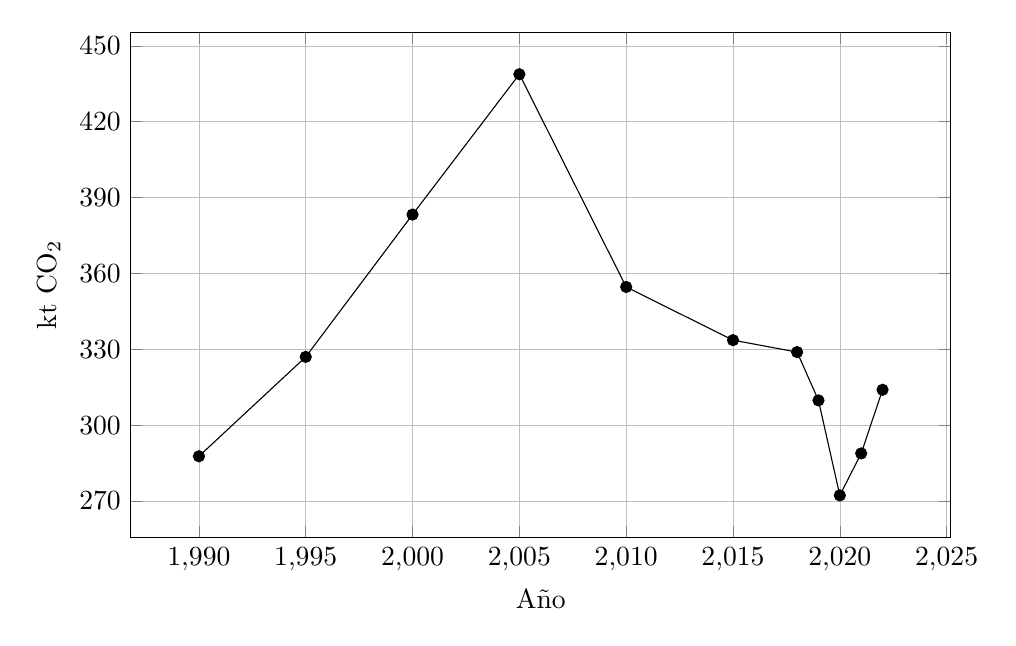
\begin{tikzpicture}
		\begin{axis}[
			xlabel={Año},
			ylabel={kt CO\textsubscript{2}},
			xtick={1990,1995,2000,2005,2010,2015,2020,2025},
			ytick={270, 300, ..., 450},
			grid=both,
			grid style={line width=.1pt, draw=gray!10},
			major grid style={line width=.2pt,draw=gray!50},
			width=12cm,
			height=8cm,
			]
			\addplot[mark=*] coordinates {
				(1990, 287.710)
				(1995, 327.011)
				(2000, 383.276)
				(2005, 438.760)
				(2010, 354.652)
				(2015, 333.623)
				(2018, 328.905)
				(2019, 309.814)
				(2020, 272.244)
				(2021, 288.848)
				(2022, 314.000)
			};
		\end{axis}
	\end{tikzpicture}

\end{figure}

En cuanto a las emisiones asociadas a la generación eléctrica:
\begin{table}[H]
	\centering
	\begin{tabular}{p{3cm}l*{11}{c}}
		\toprule
		tCO\textsubscript{2} $\times$ 1.000.000& 2011 & 2012 & 2013 & 2014 & 2015 & 2016 & 2017 & 2018 & 2019 & 2020 & 2021 & 2022 \\
		\midrule
		Carbón &   41,0 & 51,1 & 37,5 & 41,1 & 50,0 & 35,4 & 42,8 & 36,0 & 12,4 & 4,9 & 4,9 & 7,5 \\
		Fuel + Gas  &  0,0 & 0,0 & 0,0 & 0,0 & 0,0 & 0,0 & 0,0 & 0,0 & 0,0 & 0,0 & 0,0 & 0,0 \\
		Motores diésel &  2,9 & 2,9 & 2,7 & 2,6 & 2,7 & 2,8 & 2,7 & 2,2 & 2,0 & 1,6 & 1,7 & 1,7 \\
		Turbina de gas &  0,9 & 1,0 & 0,7 & 0,8 & 0,7 & 0,5 & 0,7 & 1,0 & 0,7 & 0,4 & 0,5 & 0,7 \\
		Turbina de vapor &  2,3 & 2,4 & 2,2 & 1,8 & 2,0 & 2,3 & 2,4 & 2,2 & 2,0 & 1,3 & 1,0 & 1,1 \\
		Ciclo combinado  & 21,0 & 16,4 & 11,4 & 10,5 & 12,0 & 12,0 & 14,9 & 11,8 & 21,2 & 17,1 & 17,4 & 26,2 \\
		Cogeneración  &  11,6 & 12,3 & 11,7 & 9,2 & 9,6 & 9,8 & 10,7 & 11,0 & 11,3 & 10,1 & 9,7 & 6,6 \\
		Residuos no renovables &  0,3 & 0,4 & 0,4 & 0,5 & 0,6 & 0,6 & 0,6 & 0,6 & 0,5 & 0,7 & 0,8 & 0,6 \\
		Total Emisiones &  80,1 & 86,4 & 66,6 & 66,5 & 77,6 & 63,5 & 74,9 & 64,9 & 50,0 & 36,1 & 35,9 & 44,4 \\ 
		\\
		\hline
		\\
		Factor de emision de CO\textsubscript{2} (tCO\textsubscript{2}/MWh) &  0,29 & 0,31 & 0,24 & 0,25 & 0,29 & 0,24 & 0,29 & 0,25 & 0,19 & 0,15 & 0,14 & 0,16 \\
		\bottomrule
	\end{tabular}
\end{table}

En cuanto a los rendimientos de diversas plantas de generación eléctrica:
\begin{table}[h]
	\label{tab:conversion-efficiency}
	\begin{tabular}{lcccc}
		\toprule
		&Eficiencia conversión&\multicolumn{3}{c}{Emisiones en gramos/kWh} \\
		\cline{3-5}
		&  (\%) & NOx & SO2 & CO2 \\
		\midrule
		Carbón pulverizado (sin descontaminar S) & 36 & 1.29 & 17.2 & 884 \\
		Carbón pulverizado (con descontaminación S) & 36 & 1.29 & 0.86 & 884 \\
		Carbón en lecho fluidificado & 37 & 0.42 & 0.84 & 861 \\
		Ciclo combinado de carbón gasificado & 42 & 0.11 & 0.3 & 758 \\
		Turbina de gas & 39 & 0.23 & 0 & 470 \\
		Ciclo combinado de turbina de gas & 53 & 0.1 & 0 & 345 \\
		\bottomrule
	\end{tabular}
\end{table}
\newpage
\section{Protocolo de Kioto.}
El Protocolo de Kioto estableció 3 vías para su cumplimiento:
\subsection{Políticas y medidas.}
Directiva 2033/87 CE de Comercio de Derechos de Emisión de gases
de efecto invernadero en la Unión Europea.
\subsection{Creación de sumideros.}
Se consideran sumideros todos los sistemas por los que se extraen gases de la atmósfera. Se consideran sumideros actividades como la reforestación.
\subsection{Mecanismos flexibles.}
\begin{enumerate}
	\item \textbf{Comercio de derechos de emisión (CDE):}
		Establece una asignación de una determinada cantidad de derechos de emisión gratuitos para
		las centrales térmicas y el sector industrial que equivalen a 1 tonelada de CO$_2$. Un país que haya conseguido reducir sus emisiones podrá vender a otro país que no llegue a su objetivo previsto. En España se llama \textbf{PNA} (Plan Nacional de Asignación).
	\item \textbf{Mecnismo de desarrollo limpio (MDL):}
		El país desarrollado invierte en tecnologías limpias en países en vías de desarrollo.
	\item \textbf{Aplicación conjunta (AC):}
		Un país desarrollado invierte en otro país desarrollado en un proyecto de energía limpia.
\end{enumerate}
\section{PNA.}
	La Directiva de la Unión Europea sobre Comercio de Emisiones (2003/87/CE) establece que cada Estado
	miembro deberá elaborar un Plan Nacional de Asignación (PNA) en el que se determinen la cantidad total de
	derechos a asignar durante un periodo y el procedimiento de asignación aplicado.
	
	
	Actualmente en España se asigna mediante el PNA IV donde se permiten unas emisiones de CO$_2$ = 44 MtCO$_{2-eq}$
\section{Precio de emisión.}
SENDECO2 es la plataforma que proporciona a todos los empresarios un lugar donde intercambiar Derechos de Emisión (EUAs) por Créditos de carbono (CERs) que certifican que se deja de emitir una tonelada de CO$_2$.
\subsection{Evolución del precio del derecho de emisión.}
\begin{figure}[H]
	\centering
	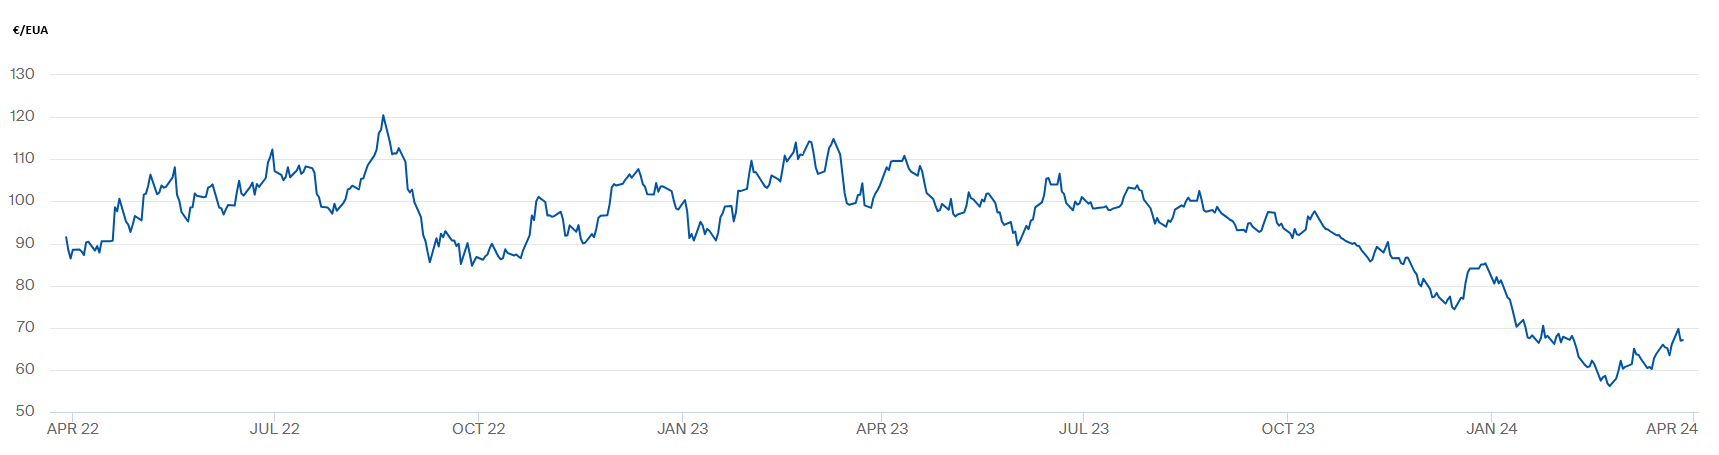
\includegraphics[width=1\linewidth]{res/tema2/precioEUA}
	\label{fig:t-emisiones}
\end{figure}
\newpage
\subsection{Influencia coste de emisión en el mercado eléctrico.}
Desde el año 2021 las centrales térmicas no tienen cantidades asignadas gratuitas y por ello, tienen que comprar derechos de emisión. Este coste repercute en el coste de la generación ofertado y, por tanto el precio de la energía como se puede ver en la figura inferior.
\begin{figure}[H]
	\centering
	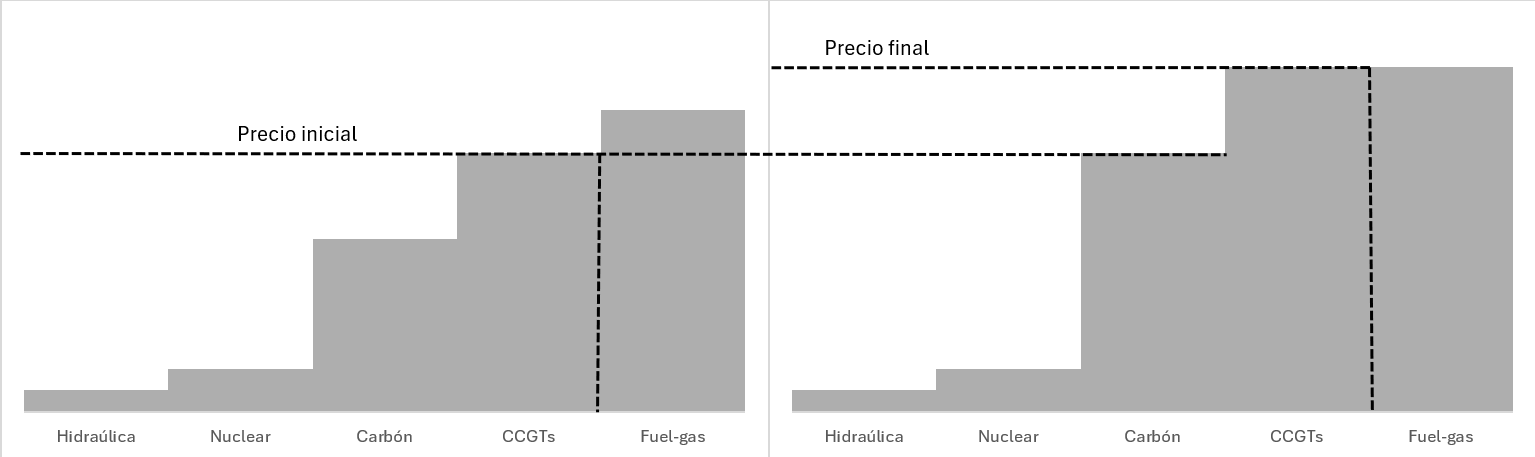
\includegraphics[width=1.2\linewidth]{res/tema2/variacionPrecio}
	\label{fig:variacionprecio}
\end{figure}
\subsection{Factor de emisión.}
El factor de emisión (fe) representa la cantidad de CO$_2$ que se genera por MWh de electricidad producida en bornes de la central:
\[fe=\frac{tCO_{2-eq}}{MWhe}=\frac{tCO_{2-eq}}{TJ}\]
Los factores de emisión se actualizan anualmente.
\subsection{Cálculo del factor de emisión.}
Para el cálculo se emplea la siguiente expresión:
\[f\left(\frac{tCO_2}{MWh}\right)=\frac{tCO_2}{TJ}\cdot\frac{3,6 TJ}{1000 MWh}\cdot\frac{100}{\eta}\]
\begin{enumerate}
	\item \textbf{Centrales térmicas de carbón:}
		El carbón es un combustible con un alto contenido en carbono y por ello genera una cantidad elevada de CO$_2$ por MWhe. El tep (tonelada equivalente petróleo) es una unidad para referir la energía con respecto a la obtenida con una tonelada de petróleo.
	\begin{table}[H]
		\centering
		\renewcommand{\arraystretch}{1.1}
		\begin{tabular}{cm{2cm}m{2cm}m{3cm}m{2cm}m{2cm}}
			\hline
			\textbf{Combustible} & \textbf{ktCO2/ktep} & \textbf{TJ/ktep} & \textbf{Factor de Emisión  combustible (tCO2/TJ)} & \textbf{Rendimiento eléctrico (\%)} & (tCO2/MWh)\\  
			\hline
			Hulla + Antracita nacional & 4,032 & 41,868 & 96,303 & 36\% & 0,96 \\
			Carbón importado           & 4,032 & 41,868 & 96,303 & 36\% & 0,96 \\
			Lignito negro              & 3,861 & 41,868 & 92,218 & 36\% & 0,92 \\
			Lignito pardo              & 3,983 & 41,868 & 95,132 & 36\% &0,95 \\ \hline
		\end{tabular}
	\end{table}
	
	\item \textbf{Centrales térmicas de ciclo combinado con gas natural:}
		Utilizan gas natural, un combustible con menor contenido en carbono que junto a su elevado rendimiento hace que tenga un menor factor de emisión.
		\begin{table}[H]
		\centering
		\renewcommand{\arraystretch}{1.1}
		\begin{tabular}{cm{2cm}m{2cm}m{3cm}m{2cm}m{2cm}}
			\hline
			\textbf{Combustible} & \textbf{ktCO2/ktep} & \textbf{TJ/ktep} & \textbf{Factor de Emisión  combustible (tCO2/TJ)} & \textbf{Rendimiento eléctrico (\%)} & (tCO2/MWh)\\  
			\hline
			Gas natural & 2,337 & 41,868 & 55,818 & 54\% & 0,37 \\
		 \hline
		\end{tabular}
	\end{table}
	\newpage
	\item \textbf{Centrales térmicas de fuel-gas:}
		Debido a su heterogeneidad se utilizan valores medios empíricos para este conjunto de centrales.
				\begin{table}[H]
			\centering
			\renewcommand{\arraystretch}{1.1}
			\begin{tabular}{cm{2cm}}
				\hline
				\textbf{Combustible}  & (tCO2/MWh)\\  
				\hline
				Gas natural & 0,77 \\
				\hline
			\end{tabular}
		\end{table}
	\item \textbf{Centrales hidráulicas, renovables y nuclear:}
		No emiten CO$_2$ para generar electricidad.
		\begin{table}[H]
			\centering
			\renewcommand{\arraystretch}{1.1}
			\begin{tabular}{cm{2cm}}
				\hline
				\textbf{Combustible}  & (tCO2/MWh)\\  
				\hline
				Centrales hidráulicas, renovables y nuclear & 0
				 \\
				\hline
			\end{tabular}
		\end{table}
	\item \textbf{Cogeneración:}
		Consiste en la producción combinada de calor y electricidad, lo que permite conseguir un rendimiento conjunto superior.
		\begin{table}[H]
			\centering
			\renewcommand{\arraystretch}{1.1}
			\begin{tabular}{cm{2cm}}
				\hline
				\textbf{Combustible}  & (tCO2/MWh)\\  
				\hline
				Cogeneración & 0,37
				\\
				\hline
			\end{tabular}
		\end{table}
	\item \textbf{Residuos:}
		Como existe una gran heterogeneidad en los combustibles empleados se toma un valor medio. En el caso de la biomasa su factor de emisión es nulo porque son neutros a nivel de emisiones. Además las emisiones de N$_2$O asociadas a los residuos no son significativas a nivel de cálculos del factor de emisión.
		\begin{table}[H]
			\centering
			\renewcommand{\arraystretch}{1.1}
			\begin{tabular}{cm{2cm}m{2cm}}
				\hline
				\textbf{Combustible} & \textbf{Rendimiento eléctrico (\%)} & (tCO2/MWh)\\  
				\hline
				Residuos &25\%& 0,24
				\\
					Biomasa &-& 0
				\\
				\hline
			\end{tabular}
		\end{table}
\end{enumerate}
\subsection{Emisiones en la combustión.}
Las fuentes de combustión que producen emisiones de CO$_2$ se calculan multiplicando el contenido de energía por un factor de emisión y oxidación (se asume igual a 1 el factor de oxidación).
\[\text{Emisiones CO}_2 = \text{Datos de la actividad} \times \text{Factor de emisión} \times \text{Factor de oxidación}\]

Los datos de actividad se expresan como el contenido de energía neto del combustible consumido [TJ] durante un periodo.
\[\text{Contenido de energía [TJ]}=\text{Combustible consumido [t o m$^3$]}\times \text{Poder calorífico combustible [TJ/t o TJ/m$^3$]}\]

El poder calorífico neto es un valor representativo de la energía liberada en la combustión en forma de calor. Esta magnitud tiene límite superior (PCS) e inferior (PCI) en función de la humedad del combustible.

\[[PCI]_s (kcal/kg)=[PCS]_s-597\cdot (9H+H_2O)\]
\begin{itemize}
	\item [-] H $\rightarrow$ \% de hidrógeno contenido en el combustible (base seca).
	\item [-] H$_2$O $\rightarrow$ \% de humedad del combustible.
\end{itemize}

\subsection{Emisiones evitadas con las energías renovables.}
Las energías renovables en España permitieron reducir la emisión de 55,6 millones de tCO$_2$ y cubrieron el 42,2\% de la demanda eléctrica.
\newpage
\section{Combustibles fósiles.}
\subsection{Combustible sólidos.}
\begin{enumerate}
	\item \textbf{Biomasa:}
		El combustible esta compuesto de materia vegetal que había sido creada a través de la fotosíntesis:
		\[6 CO_2 + 6 H_2O + 112 kcal/mol \rightarrow C_6 (H_2O)_6 + 6 O_2 ( Glucosa)\]
		Por tanto, la fotosíntesis fija al año 18.000 Mt de CO$_2$ y por tanto, quemar esta planta no produce más CO$_2$ que el que liberaría al morir por fermentación. De esta manera, se podría considerar renovable.
	\item \textbf{Carbón:}
		Es una roca de fácil combustión con aproximadamente el 50\% del peso en carbono. No obstante, en función del porcentaje de carbono cambia el poder calorífico:
		\begin{table}[H]
			\centering
			\renewcommand{\arraystretch}{1.1}
			\begin{tabular}{cccc}
				\hline
				&\textbf{Lignito} & \textbf{Hulla} & \textbf{Antracita}\\  
				\hline
			Densidad &  1,1-1,3&1,2-1,5  &1,4-1,8\\ 
			Humedad (\%) &20-50  &3-25  &3-5\\ 
			\% C & 27-31 &  37-86&89-98\\ 
			\% Volátiles &25-55  &25-50  &2-14\\ 
			PC (kcal/kg) &  2000-4000&3500-7500  &7000-8350\\ 
				\hline
			\end{tabular}
		\end{table}
		De manera general en función del tipo de carbón el combustible tiene distintas propiedades:
		\begin{enumerate}
			\item \textbf{Lignito:}
			posee un color parduzco o negro. Por lo general tiene un alto contenido en volátiles. El lignito
			negro, o carbón subbituminoso, es duro y su humedad está limitada.
			Los lignitos españoles son altamente sulfurosos. El lignito
			pardo es un carbón terroso, con alto contenido en humedad.
			\item \textbf{Hulla:}
			carbón bituminoso o carbón graso. Abarca una amplia variedad de carbones.
			Es más blando que la antracita. Arde con llama humeante y larga. Su aspecto varía desde el pardo oscuro hasta
			el negro. Son los carbones que presentan un mayor interés para la generación eléctrica.
			\item \textbf{Antracita:}
			también llamado carbón de piedra o carbón duro. De gran contenido en carbono fijo. Es duro y negro. Tiene lustre semimetálico y fractura semiconcoidal. Arde con llama azul y
			corta, sin apenas humo.
		\end{enumerate}
		El carbón esta formado por distintos elementos que condicionan su comportamiento como combustible:
		\begin{enumerate}
			\item \textbf{Carbón fijo (65-95\%):}
				A mayor porcentaje mayor poder calorífico. Permite estimar el porcentaje de generación de CO$_2$.
			\item \textbf{Hidrógeno (3-6\%):}
				Aumenta el poder calorífico y facilita la combustión.
			\item \textbf{Azufre (0,2-11\%):}
				Los carbones con alto contenido en azufre deben ser tratados porque generan SO$_2$ $\rightarrow$SO$_3$ que es altamente contaminante al provocar lluvias ácidas y ser peligroso para el ser humano.
				
				
				Los tratamientos normalmente empleados para reducir el porcentaje de azufre son:
				\begin{itemize}
					\item [-] Lavaderos de carbón: Antes de la combustión.
					\item [-] Adición de caliza: Durante la combustión (\textbf{solo lecho fluido y gasificación}).
					\item [-] Desulfuración de los gases: Después de la combustión.
				\end{itemize}
			\item \textbf{Humedad (1-60\%):}
				Provoca una disminución del poder calorífico y del rendimiento. Además necesita aire más caliente y puede provocar atascos en las tolvas.
			\item \textbf{Nitrógeno (1-1,5\%):}
				Provoca la formación de NOx en función de la temperatura de combustión.
			\item \textbf{Oxígeno (2-30\%):}
				Sirve como medida del grado de oxidación y permite reducir la cantidad de aire a aportar.
				\newpage
			\item \textbf{Materia volátil (5-40\%):}
				Se desprende durante la fase inicial del proceso de combustión, facilitan la ignición. A mayor materia volátil mayor será el humo producido.
				\begin{itemize}
					\item [-] Si tienen mucha materia volátil dan llamas cortas , calientes y muy estables. Hay pocos inquemados.
					\item [-] Si tienen poca materia volátil dan llamas largas e inestables. Se necesitan fuegos opuestos para elevar la temperatura de llama u hogares de arco que
					soporten llamas muy largas. Necesita molienda muy fina.
				\end{itemize}
			\item \textbf{Cenizas (30\%):}
				Materiales minerales no volátiles. Son residuos tras la combustión completa. Reducen la calidad del carbón.		
		\end{enumerate}
		\textbf{Combustión del carbón:} Es una reacción de oxidación con fuente de ignición donde el oxígeno se combina con el combustible para formar óxidos liberando gran cantidad de calor.
		\begin{itemize}
			\item [-] Para favorecer la combustión se pulveriza el carbón.
			\item [-] \textbf{Reacciones principales:}
			\[C+O_2\rightarrow CO_2 + 8100kcal/kg \ de \ C\]
			\[C+0,5O_2\rightarrow CO +2500kcal/kg \ de \ C\]
			\[H_2+0,5O_2\rightarrow H_2O +33600kcal/kg \ de \ H_2\]
			\[S+O_2\rightarrow SO_2 +2500kcal/kg \ de \ S\]
			\[N+O_2\rightarrow NO+O\]
			\item [-] \textbf{Condiciones necesarias combustión completa:}
			\begin{itemize}
				\item Cantidad suficiente de aire (con algo de exceso).
				\item Procurar buen grado de mezcla entre comburente y combustible (pulverización).
				\item Tiempo de residencia suficiente.
				\item Garantizar temperatura mínima en el hogar.
			\end{itemize}
			\item [-] Se considera que la combustión tiene lugar cuando la velocidad de oxidación es suficiente como para automantenerse. Cuando la velocidad de alimentación del combustible y comburente iguala a la velocidad de
			propagación de la llama entonces se estabiliza.
			\item [-]La caldera más común es la de carbón pulverizado. El diseño de estas depende del carbón a quemar.
			\begin{itemize}
				\item 240 minutos para plena carga en arranque en frío.
				\item 120 minutos para plena carga en arranque en templado (24h parada).
				\item 70 minutos para plena carga en arranque en caliente (8h parada).
				\item 60 minutos para plena carga en rearranque (2h parada).
			\end{itemize}
			\item [-] \textbf{Tipos de combustiones:} Desde el punto de vista estequiométrico puede ser completa o incompleta.
			\begin{itemize}
				\item Se considera completa cuando el combustible no quemado no supera el 2\%.
				\begin{itemize}
					\item 13 Nm$^3$ de aire por kg de carbono.
				\end{itemize}
				\item En la combustión incompleta se emite CO.
			\end{itemize}
			Se controla el tipo de combustión mediante la medida de gases a la salida de la chimenea.
			\begin{itemize}
				\item Índice emisión: 
				\[EI=\frac{\text{masa de gases emitidos}}{\text{masa de combustible quemado}}\]
				\item Masa de contaminante emitida por unidad de combustible quemado: 
				\[M/ud= \frac{EI}{Hc} (gr/MJ)\]
				\item Indice inmisión: emisión a 2m de altura sobre el suelo.
			\end{itemize}
			\item [-] \textbf{Combustión con exceso de aire:}
				Para evitar la formación de inquemados sólidos se procura una mezcla homogénea y se introduce un exceso de caudal. Para ello, se definen el exceso de aire porcentual (EA) y el coeficiente de exceso de aire (n):
				\[EA(\%)=100\times\frac{A_{exp}-A_{teorico}}{A_{teorico}}=100\times(n-1)\]
				No obstante, aumentar demasiado el exceso de aire provoca que se pierda parte del calor de la caldera.
				\begin{table}[H]
					\centering
					\renewcommand{\arraystretch}{1.1}
					\begin{tabular}{cc}
						\hline
						\textbf{Combustible}&\textbf{n}\\  
						\hline
						Gaseoso& 1,1-1,2\\
						Líquido & 1,15-1,3\\
						Pulverizado & 1,15-1,5\\ 
						\hline
					\end{tabular}
				\end{table}
				Para conocer el exceso de aire a emplear se emplea el diagrama de Oswald a partir de los contenidos de CO y CO$_2$. La región de trabajo óptima se situa en torno al 13\% de CO$_2$ en los gases de combustión.
				\begin{figure}[H]
					\begin{minipage}{0.6\linewidth}
						\centering
						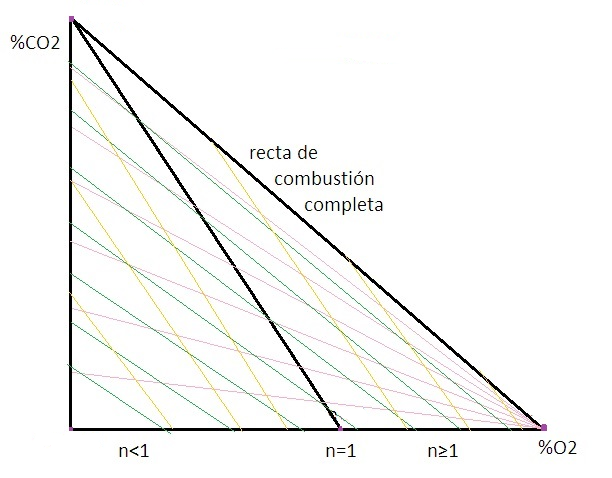
\includegraphics[width=\linewidth]{res/tema2/oswaldo}
						\label{fig:oswaldo}
					\end{minipage}%
					\begin{minipage}{0.4\linewidth}
						\centering
						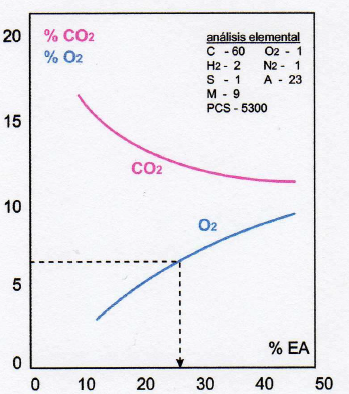
\includegraphics[width=\linewidth]{res/tema2/CO2O2}
						\label{fig:co2o2}
					\end{minipage}
				\end{figure}
				\item [-] \textbf{Balance energético en la caldera:} Se deben tener en cuenta las características energéticas y gasto del combustible frente a la calidad del vapor generado.
				
				
				Las principales pérdidas de calor en la caldera se deben a:
				\begin{itemize}
					\item Combustión incompleta: Se reduce a medida que se aumenta el exceso de aire.
					\item Calor sensible de los gases de escape: Aumenta a medida que se aumenta el exceso de aire.
					\item Sólidos inquemados: Disminuye a medida que se aumenta el exceso de aire.
				\end{itemize}
				Que resumido en un gráfico queda:
				\begin{figure}[H]
					\centering
					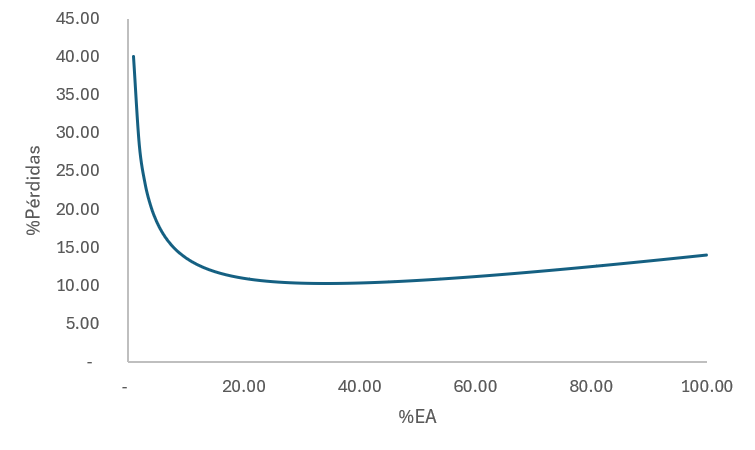
\includegraphics[width=0.5\linewidth]{res/tema2/perdidas}
					\label{fig:perdidas}
				\end{figure}
				Por tanto, el rendimiento de la caldera queda como:
				\[\eta = \frac{\text{Potencia térmica cedida al vapor sobrecalentado de salida}}{PCI \times \dot{m}_\text{combustible} \times \text{Potencia térmica aire caliente}}\approx 85-88\%\]
				En general en la caldera hay varios rendimientos:
				\begin{figure}[H]
					\centering
					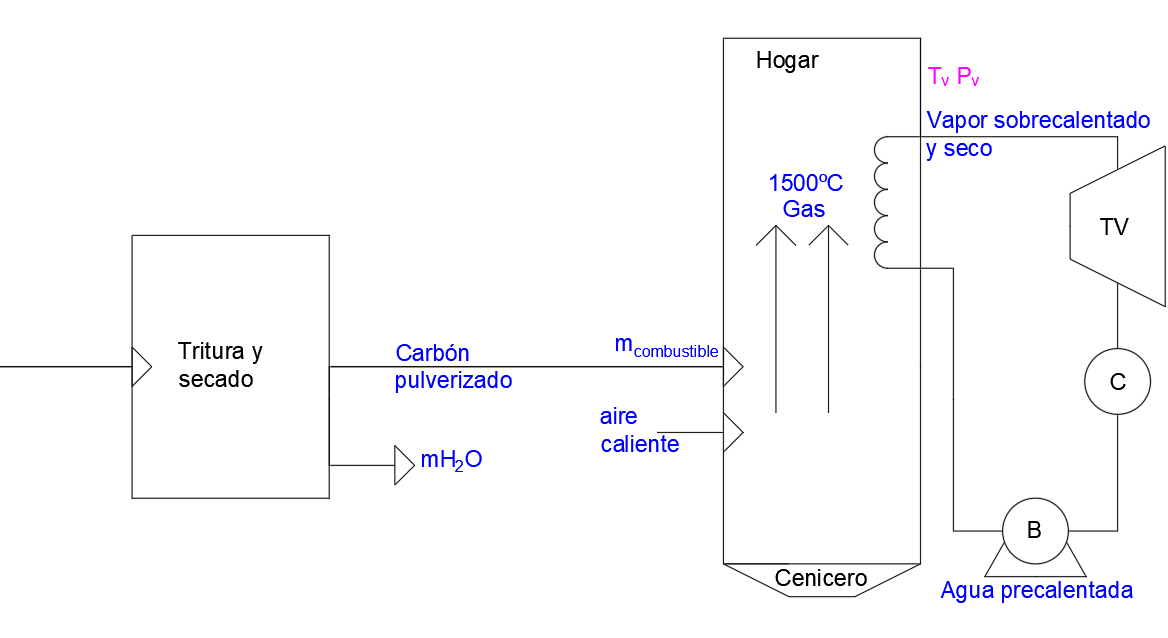
\includegraphics[width=0.7\linewidth]{res/tema2/caldera}
					\label{fig:caldera}
				\end{figure}
				Los distintos rendimientos son:
				\[\eta_{caldera}=\frac{P_{tv}}{P_{tv}+P_{aire}}\]
				\[P_{tv}=\dot{m}_{comb}\times PCI\]
				\[P_{aire}=\dot{m}_{aire}\times h_{aire}\]
				\[\eta_{planta}=\frac{P_{bc}}{P_{comb}}\]
		\end{itemize}
\end{enumerate}
\subsection{Combustible gaseosos.}
Principalmente gases naturales y materia volátil. Son de fácil combustión (poco exceso de aire). Emiten NO$_x$ y SO$_2$. Tienen peligro de explosión y por ello, requieren elevada estanqueidad.
\subsection{Combustible líquidos.}
Se compone de mezclas complejas de hidrocarburos de cadena larga. Tienen un punto de inflamación baja. Emiten NO$_x$ y SO$_2$. Provocan corrosión a baja temperatura.

\section{Impacto ambiental de las centrales térmicas de combustión.}
\subsection{Composición de gases de la combustión.}
\begin{enumerate}
	\item \textbf{Monóxido de carbono (CO):}
		Se produce por combustiones incompletas de compuestos que contienen carbono. Es un gas muy tóxico. En contacto con el oxígeno forma CO$_2$.
	\item \textbf{Materia particulada (PM):}
		Son mineral, inquemados y elementos de traza.
		\begin{itemize}
			\item [-] Una cuarta parte se recoge como ceniza mediante los ceniceros. El resto es liberado y se captura con filtros ciclónicos o electrostáticos.
			\item [-] Los elementos de traza (Hg y Se) se capturan mediante filtros de resinas.
		\end{itemize}
		Los minerales que se consideran contaminantes son:  Be, Cr, Mn, Co, Ni, As, Se, Cd, Sb, Hg y Pb.
	\item \textbf{Compuestos orgánicos:}
		Se pueden encontrar como gas si son volátiles (metano y benceno) o en la superficie de partículas como hidrocarburos aromáticos policlínicos.
	\item \textbf{Óxidos de azufre (SO$_2$, SO$_3$, SH$_2$):}
		Provocan lluvia ácida. En las calderas se forma SO$_2$ que posteriormente forma el resto de óxidos.
		\begin{figure}[H]
			\centering
			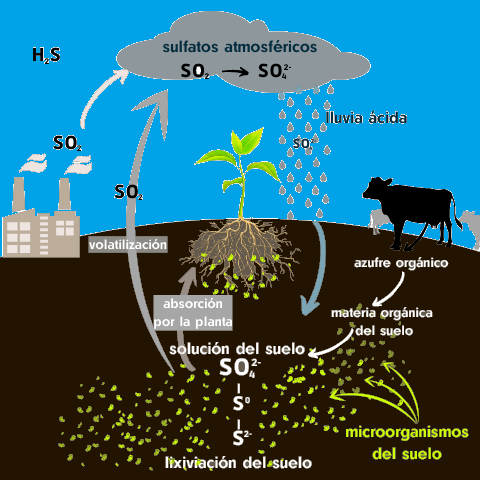
\includegraphics[width=0.4\linewidth]{res/tema2/sicloazufgre}
			\label{fig:sicloazufgre}
		\end{figure}
		
	\item \textbf{Óxidos de nitrógeno (NO$_x$):}
		Provocan lluvia ácida, destrucción de la capa de ozono y smog fotoquímico:
		\begin{itemize}
			\item [-] \textbf{NO$_2$:} precursor del efecto invernadero. Son muy absorbentes de radiación infrarroja. Se genera a partir del NO con exceso de oxígeno.
			\item [-] \textbf{NO:} reducción del ozono en la estratosfera (es menos tóxico que el NO$_2$). Se genera por la alta temperatura de la caldera con el N$_2$ del aire. 
			\item [-] \textbf{N$_2$O:} reducción del ozono en la troposfera. Se produce en mezclas pobres con poco O$_2$.
		\end{itemize}
\end{enumerate}
\subsection{Tratamientos para reducción de emisiones.}
\begin{enumerate}
	\item \textbf{Óxidos de azufre (SO$_2$):}
	Se clasifican en función del momento de la combustión en el que se realice el tratamiento:
	\begin{enumerate}
		\item \textbf{Precombustión:} 
		\begin{itemize}
			\item [-] Uso de carbones de alta calidad.
			\item [-] Combustión mixta con gas natural.
			\item [-] Lavado y desulfuración del combustible.
			\item [-] Gasificación del carbón.
		\end{itemize}
		\item \textbf{Durante la combustión:}
		\textbf{Solo en calderas de lecho fluidificado} se puede introducir caliza CaCO$_3$ para fijar el azufre. 
		\item \textbf{Postcombustión:}
			Se manipulan los gases mediante torres de lavado por vía húmeda o semihumeda con un rendimiento del 40\%.
			
			El proceso de absorción química en las torres de lavado es el siguiente:
			\[SO_2+H_2O\rightarrow H_2SO_4\]
			\[CaCO_3+H_2SO_4\rightarrow CaSO_3+CO_2+H_2O\]
			\[CaSO_3+0,5O_2+H_2O\rightarrow CaSO_4+2H_2O\]
			\begin{figure}[H]
				\centering
				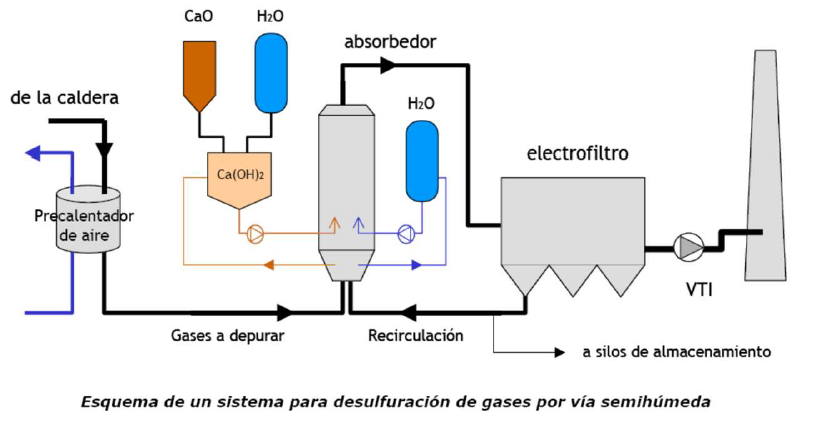
\includegraphics[width=0.5\linewidth]{res/tema2/desulfuric}
				\label{fig:desulfuric}
			\end{figure}
			
	\end{enumerate}
	\item \textbf{Óxidos de nitrógeno (NO$_x$):}
	\begin{itemize}
		\item [-] \textbf{Técnicas primarias:} Se basan en el control del proceso de combustión. Modificacando los siguientes parámetros que reducen las emisiones de NO$_x$ a costa del rendimiento:
		\begin{itemize}
			\item Reducción de la temperatura.
			\item Disminución del exceso de aire.
			\item Inyección de vapor.
			\item Combustión con O$_2$ puro.
			\item Combustible con menos N$_2$.
			\item Uso de catalizadores.
		\end{itemize}
		El problema de los NO$_x$ disminuye en las calderas de lecho fluido debido a que trabajan a 900° C en lugar de los 1500° C de una caldera convencional.
		\item [-] \textbf{Técnicas secundarias:} Se basan en reducir las emisiones de gases tras la combustión:
		\begin{itemize}
			\item Absorción química con $H_2SO_4$:
			
\begin{figure}[H]
	\centering
	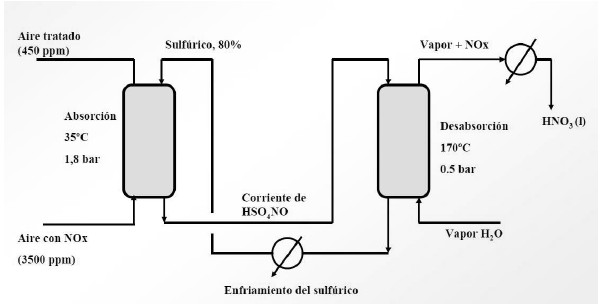
\includegraphics[width=0.5\linewidth]{res/tema2/H2so4abs}
	\label{fig:h2so4abs}
\end{figure}
	\item Proceso TYCO: incorpora eliminación $SO_2$ y recupera ácidos:
	
\begin{figure}[H]
	\centering
	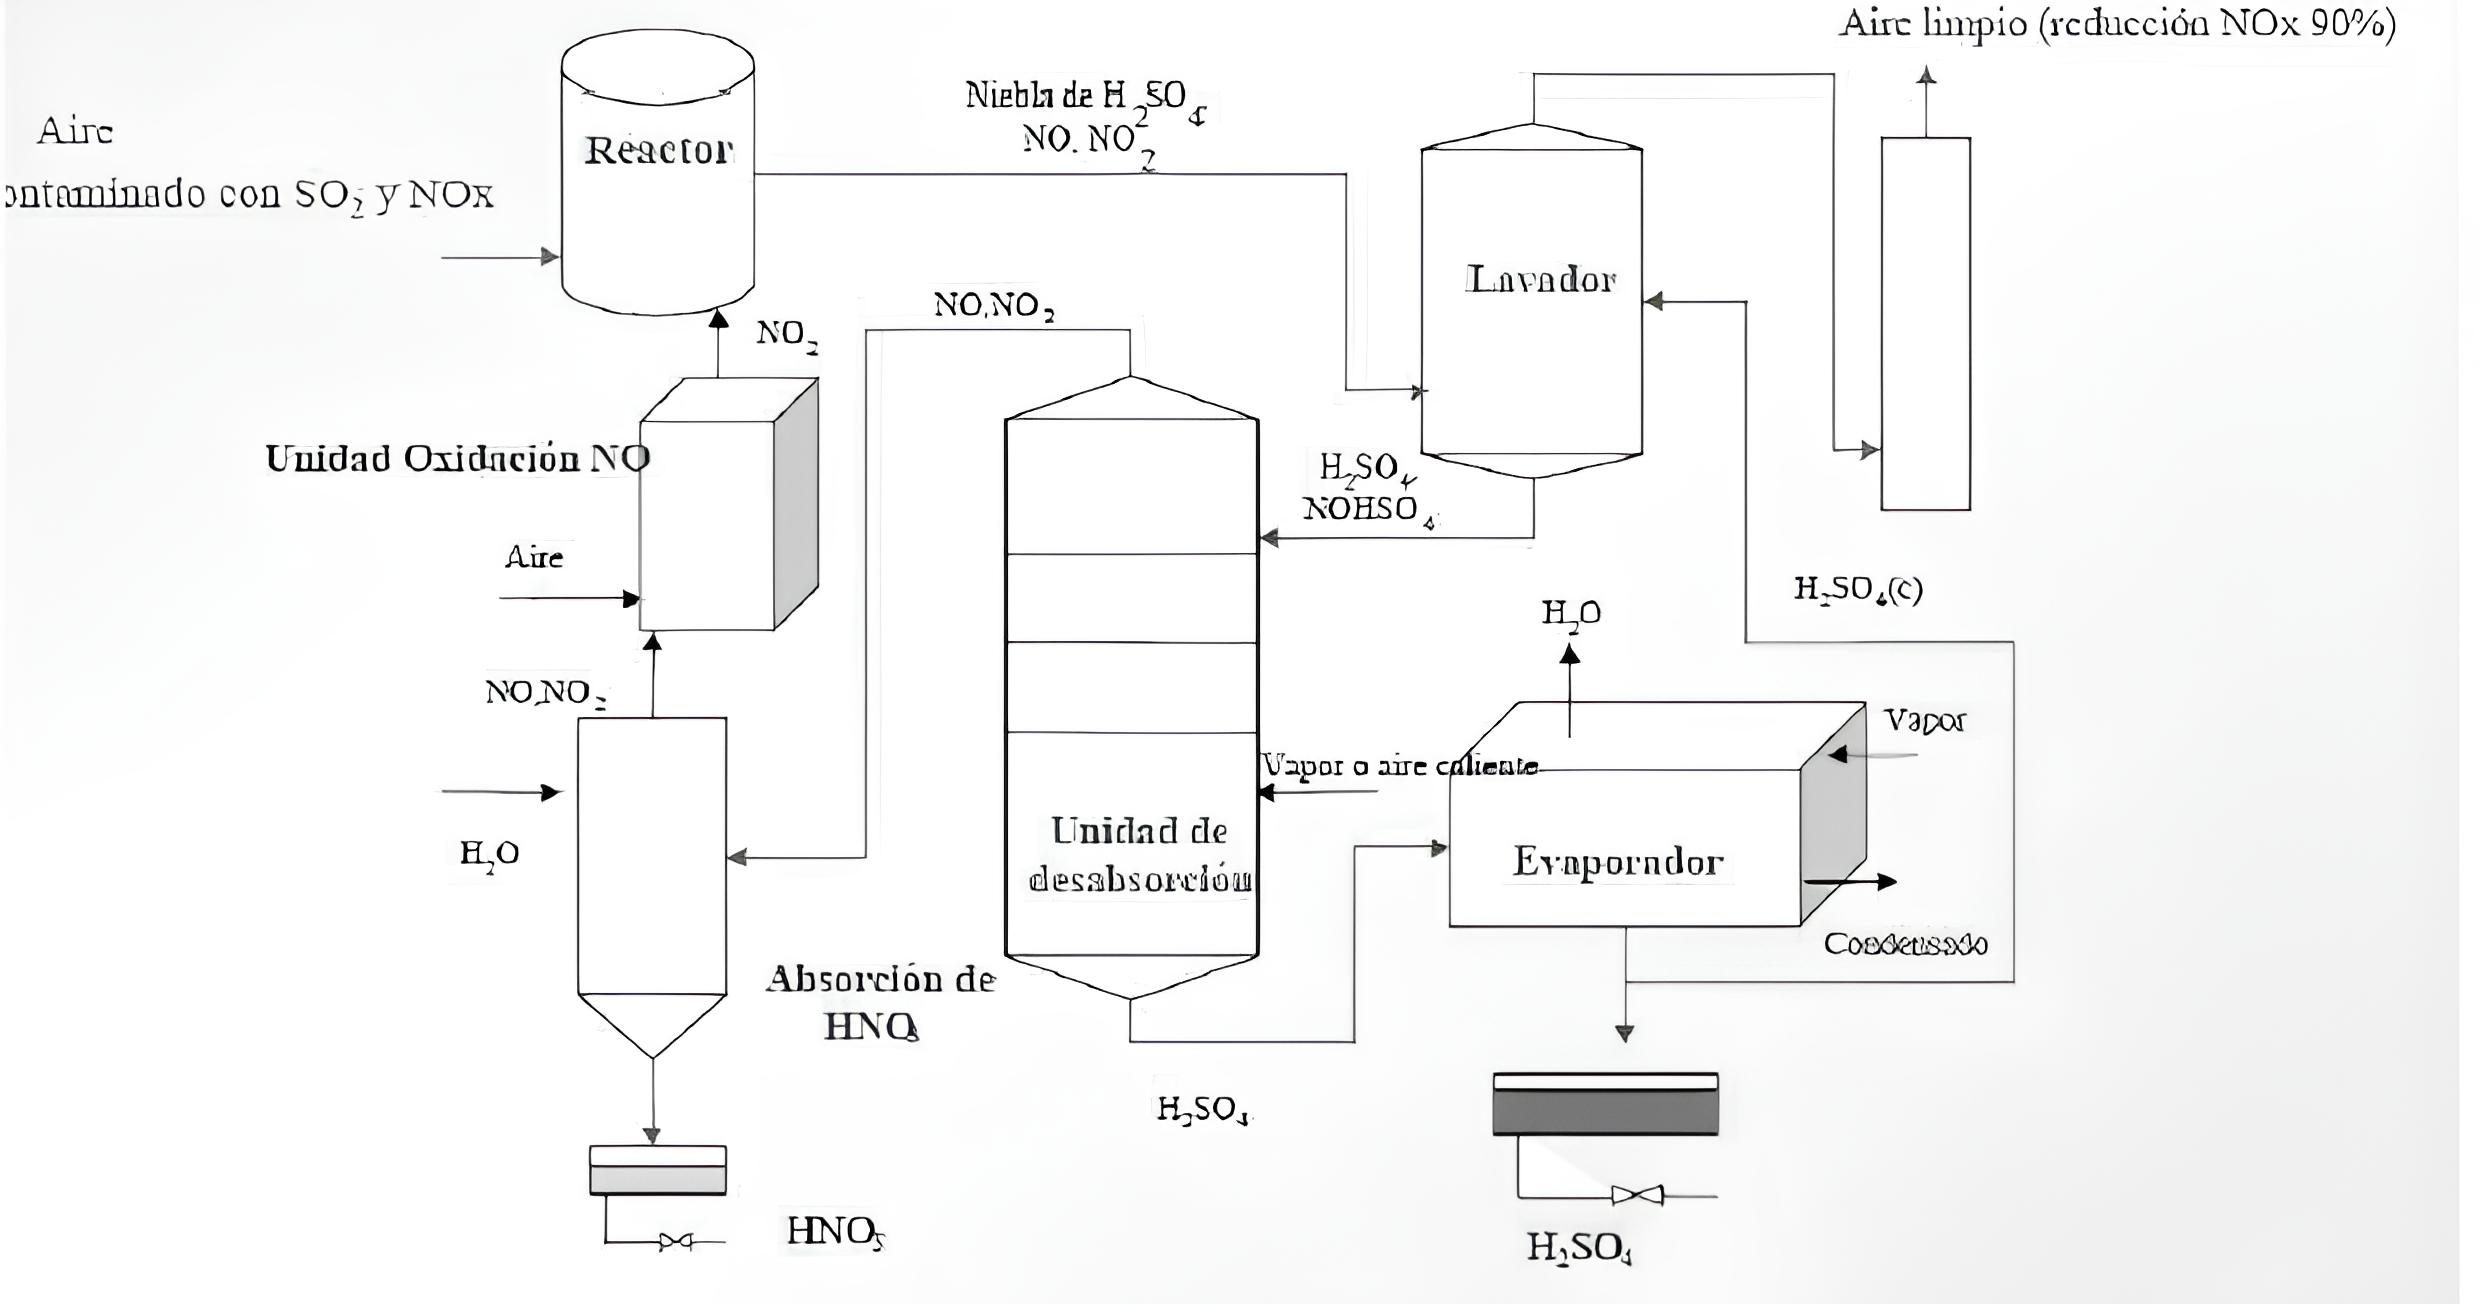
\includegraphics[width=0.5\linewidth]{res/tema2/tyci+}
	\label{fig:tyci}
\end{figure}
\item Reducción catalítica selectiva: se emplea amoniaco que al reaccionar con los NO$_x$. Tiene una eficiencia de eliminación del 85\%.
\[6NO_x+4xNH_3\rightarrow [2x+3]N_2+6xH_2O\]
		\end{itemize}
	\end{itemize}
	\item \textbf{Materia particulada (PM):} Se trata mediante filtros ciclónicos y electrostáticos tras la combustión. Tienen un gran consumo energético 12\% del autoconsumo.
\end{enumerate}
\begin{figure}[H]
	\centering
	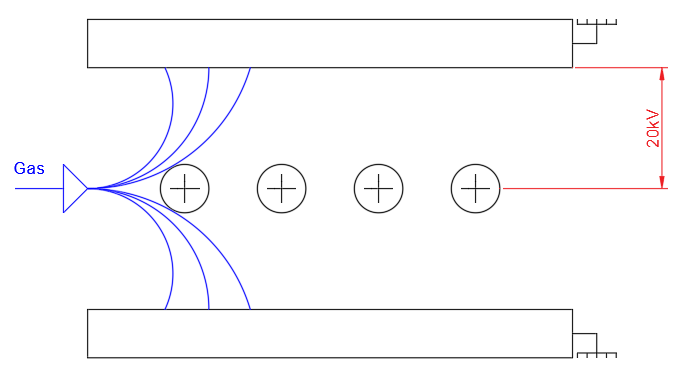
\includegraphics[width=0.7\linewidth]{res/tema2/filtroelectrostatico}
	\label{fig:filtroelectrostatico}
\end{figure}

\subsection{Impacto ambiental centrales térmicas.}
Anteriormente se han discutido principalmente las centrales térmicas de carbón, pero si el combustible es líquido o sólido cambia ligeramente el impacto ambiental.
\begin{itemize}
	\item \textbf{Combustible líquido:}
		El impacto ambiental es menor que el de las de carbón aunque el uso de estas centrales esta disminuyendo. Emite menos gases contaminantes y la materia particulada esta compuesta principalmente por hollín. 
		
		
		Los combustibles principales usados son los gasóleos (comparten mercado con la automoción) y los fuelóleos (uso exclusivo en instalaciones térmicas).
		
		El principal inconveniente de los fuelóleos es su alto contenido en azufre.
	\item \textbf{Gas natural:}
		El gas natural es un combustible con muy alto poder calorífico y son las centrales de combustión de combustibles fósiles con menor impacto ambiental aunque tienen problemas de emisiones de NO$_x$ y generan elevada contaminación acústica.
		
		Cabe destacar, que otra ventaja es que como se recibe continuamente gas no es necesario invertir en sistemas de almacenamiento y, además, no necesita tratamiento previo. Que también como durante el transporte se entierran la contaminación producida por fugas es despreciable.
\end{itemize}
\section{Impacto ambiental centrales nucleares.}
Tienen el mismo impacto térmico y químico que las centrales térmicas convencionales aunque no libera gases contaminantes. No obstante, presenta el problema de los residuos radioactivos.
\subsection{Tipos de radioactividad.}
La radioactividad es un efecto producido por descomposición espontánea de un núcleo inestable en otro más estable. Los tipos de radiación principales son:
\begin{itemize}
	\item [-] La radiación alfa ($\alpha$) está formada por núcleos de helio. No es capaz de atravesar el papel.
	\item [-] La radiación beta ($\beta$) está constituida por electrones. No es capaz de atravesar el acero.
	\item [-] La radiación gamma ($\gamma$) es de naturaleza electromagnética. No es capaz de atravesar el plomo.
	\item [-] Radiación neutrónica (n). No es capaz de atravesar el cemento.
\end{itemize}
\subsection{Medida de la radioactividad.}
Se mide mediante la cantidad de radiación emitida. 
\begin{itemize}
	\item [-] Si la radiación afecta al ser humano se mide en Sievert (Sv): Unidad de dosis equivalente.
	\item [-] Si la radiación afecta a un objeto se mide en Gray (Gy): Unidad de dosis absorbida. Se define como la dosis de radiación que transfiere una energía de 1 julio a 1 kilogramo masa de
	material irradiado
	\item [-] Si se habla de fuente emisora de radiación (material radiactivo) se emplea el Becquerel (Bq). Se define como la actividad de un material que experimenta una desintegración por segundo.
	
\begin{figure}[H]
	\begin{center}
	\scalebox{0.8}[0.8]{
		\begin{tikzpicture}
			\def\printonlylargeenough#1#2{\unless\ifdim#2pt<#1pt\relax
				#2\printnumbertrue
				\else
				\printnumberfalse
				\fi}
			\newif\ifprintnumber
			\pie[rotate=90, text=legend, before number=\printonlylargeenough{1}, after number=\ifprintnumber\%\fi]{
				36.7/Inhalación de radón,
				29.1/Aplicaciones médicas,
				13.1/Radiación suelo,
				10.2/Radiación cosmica,
				9.9/Propio Cuerpo,
				0.6/Exposición profesional: 0.6\%,
				0.3/Poso radioactivo 0.3\%,
				0.1/Centrales nucleares 0.1\%
			}
		\end{tikzpicture}
}	\end{center}
\end{figure}	
\end{itemize}
\subsection{Clasificación de los residuos radioactivos.}
\begin{itemize}
	\item [-] \textbf{Según el estado de agregación.}
	\begin{enumerate}
		\item \textbf{Residuos gaseosos:} Se debe distinguir entre isotopos radioactivos y el aire. Mediante filtros de alta eficiencia (HEPA) se retiene el 99,9\% de las partículas de 0,3 $\mu$m.
		\item \textbf{Residuos líquidos:} Principalmente tritio. Se eliminan con operaciones de filtración, centrifugación, precipitación química,
		intercambio iónico y evaporación .
		\item \textbf{Residuos sólidos:} Se clasifican en alta, media o baja actividad.
	\end{enumerate}
	\item [-] \textbf{Según la radiactividad.}
	\begin{enumerate}
		\item \textbf{Sólidos de actividad media y baja:} Tienen una vida media de menos de 30 años. Se mezclan con aglomerantes y se almacenan en depósitos. 
		
		España genera 1220 m$^3$ al año. Los residuos dejan de ser peligrosos a los cientos de años con lo cual es seguro almacenarlos en instalaciones permanentes en superficie. 
		\item \textbf{Sólidos de alta actividad:} Están constituidos por el combustible gastado. Contienen radionucleidos de larga vida media que tardan miles de años en llegar a niveles seguros de radiación. 
		
		Se enfrían en piscinas en la propia central durante 5 años y después se embuten en vidrio para ser almacenados en lugares de almacenamiento centralizado. Actualmente en España estos residuos se almacenan en el extranjero con un coste de 49.545,17€/día (en teoria deberian haber vuelto a España en 2010).
	\end{enumerate}
	La generación media de una central tipo de 1.000 MW es de 20 toneladas de uranio al
	año (combustible gastado), de 50 m$_3$ (centrales con tecnología PWR) y 130 m$^3$
	(centrales BWR) de residuos de media y baja actividad.
	
	Anteriormente el precio de la gestión de los residuos radiactivos recaía sobre el consumidor de la energía eléctrica. No obstante, actualmente se plantea que las nucleares paguen esta gestión.
\end{itemize}
\subsection{Gestión del combustible gastado.}
Cuando se descarga el combustible del reactor todavía hay gran cantidad de energía puede ser utilizada al solo haberse gastado el 5\% de la energía inicial.
\begin{itemize}
	\item [-] Si se almacena tras su uso en instalaciones de almacenamiento geológico profundo se habla de ciclo abierto.
	\item [-] Si se reprocesa el combustible gastado para ser reutilizado se habla de ciclo cerrado. En el ciclo cerrado se recupera el combustible fabricando pastillas de óxido de uranio (UO$_2$) y óxido de plutonio (PuO$_2$) que se denominan combustible MOX.
\end{itemize}
Las piscinas donde se almacena el combustible gastado suelen ser de agua por su alto coeficiente de transmisión del calor y sus propiedades como blindaje. Hoy en día presentan una problemática debido a que las piscinas de las centrales nucleares españolas están saturadas.
\section{Impacto ambiental centrales hidroeléctricas.}
De acuerdo con la IHA (International Hydropower Association), existen varios aspectos clave que hay que tener en
cuenta para mantener el potencial hidroeléctrico con un desarrollo sostenible en materia medioambiental:
\begin{enumerate}
	\item \textbf{Calidad del agua:} Puede reducir la cantidad de oxígeno en agua, su temperatura y la estratificación de los sedimentos.
	\item \textbf{Erosión y transporte de sedimentos:} Cambia la cantidad de sedimentos transportados y a largo plazo puede cambiar la forma del río por el cambio de la erosión.
	\item \textbf{Hidrología y flujos mediambientales del río:} Como cambia la hidrología y el entorno del río afecta a la fauna y a actividades humanas que se desarrollaban en el río.
	\item \textbf{Especies en peligro de extinción:}  La construcción de una presa puede poner en serio riesgo a especies amenazadas o únicas, debido a los
	cambios del hábitat natural.
	\item \textbf{Paso de especies:} Muchas especies recorren el río a lo largo de su ciclo de vida en uno o ambos sentidos. En muchos lugares,
	la migración de peces (como el salmón) es un acontecimiento anual, que se ve seriamente dificultado por las
	presas.
	\item \textbf{Plagas animales y vegetales en los embalses:} Los cambios en las condiciones del agua pueden facilitar la colonización de especies
	ajenas al entorno, creando plagas.
	\item \textbf{Aspectos sanitarios:} Los cambios producidos en el entorno por la construcción de presas pueden afectar a la salud pública,
	influyendo en la transmisión de enfermedades.
	\item \textbf{Actividades de construcción:} Las actividades de construcción provocan alteraciones en el medio acuático y terrestre.
\end{enumerate}
\section{Impacto ambiental transporte y transformación energía eléctrica.}
Tienen un impacto menor que las instalaciones de producción.
\begin{enumerate}
	\item \textbf{Líneas de transporte y distribución:} Se utilizan terrenos para la instalación de torres que provocan impacto visual y afectan a la avifauna.
	\item \textbf{Subestaciones de transformación:}
	Provocan una pérdida de suelo y vegetación, emiten ruidos y pueden provocar contaminación de agua por fugas.
	\item \textbf{Redes de baja tensión y centros de transformación:} Producen impacto visual y emisión de ruidos.
	\item \textbf{Campos electromagnéticos:} Los campos eléctricos son proporcionales a la tensión y los campos magnéticos a la intensidad.	
\end{enumerate}